\documentclass[portrait, a1paper, fontscale=0.5]{baposter}

\usepackage[utf8]{inputenc}
\usepackage{graphicx}

\definecolor{bgcolorone}{RGB}{225,225,225}
\definecolor{bgcolortwo}{RGB}{225,225,225}
\definecolor{bordercolor}{RGB}{153,153,153}
\definecolor{headercolorone}{RGB}{255,255,255}
\definecolor{headercolortwo}{RGB}{255,255,255}
\definecolor{headerfontcolor}{RGB}{7,67,145}
\definecolor{boxcolorone}{RGB}{200,200,200}

\pdfinfo
{
	/Title (SNA)
	/Author (P. Kus, P. Karban, F. Mach)
}

\begin{document}

\background{}

\begin{poster}{
	grid=false,
	columns=6,
	background=plain,
	bgColorOne=bgcolorone,
	%bgColorTwo=bgcolortwo,
	borderColor=bordercolor,
	headerColorOne=headercolorone,
	headerColorTwo=headercolortwo,
	headerFontColor=headerfontcolor,
	boxColorOne=boxcolorone,
	headershape=roundedright,
	headerfont=\large\sc,
	textborder=roundedleft,
	background=user,
	headerborder=open,
	boxshade=none
}
{
\includegraphics[width=17em]{fel.pdf}}
{\huge\textsc{\textcolor{headerfontcolor}{Solving nonlinear coupled problems using Agros2D}}\vspace{0.75em}}
{\Large{\textcolor{headerfontcolor}{P. Kus$^{1}$, P. Karban$^{2}$ and F. Mach$^{1, 2}$\\{\large $^{1}$ \textit{Institute of Thermomechanics, Academy of Sciences CR, v. v. i.}}\\{\large $^{2}$ \textit{Faculty of Electrical Engineering, University of West Bohemia}}}}}
{
\includegraphics[width=7em]{it.png}}

\headerbox{About Agros2D}{name=about,column=0,row=0, span=2}{
Agros2D is a multiplatform C++ application for the solution of partial differential equations (PDE) based on the Hermes library, developed by the hpfem.org group at the University of West Bohemia in Pilsen. Hermes library is developed at University od Reno in Nevada. Agros2D is distributed under the GNU General Public License.
}

\headerbox{Supported physical fields}{name=fields,column=0,row=0, span=2,below=about}{
\begin{itemize} \itemsep1pt \parskip0pt \parsep0pt
\item Electrostatic fields
\item Electric current fields
\item Magnetic fields (steady state, harmonic and transient analysis)
\item High frequency electromagnetic fields - in development
\item Temperature fields (steady state and transient analysis)
\item Acoustic field (harmonic and transient analysis)
\item Linear thermo-elasticity
\item Incompressible flow (steady state and transient analysis) - in development
\end{itemize}
}

\headerbox{Key Features}{name=features,column=0,row=0,span=2,below=fields}{
\begin{itemize} \itemsep1pt \parskip0pt \parsep0pt
\item Steady state, transient and harmonic analysis
\item Curvilinear elements
\item Arbitrary level hanging nodes
\item Multimesh assembling
\item Automatic hp-adaptivity
\end{itemize}
}

\headerbox{Simple GUI control}{name=gui,column=0,row=0,span=2,below=features}{
\begin{itemize} \itemsep1pt \parskip0pt \parsep0pt
\item Interactive geometry definition
\item AutoCAD DXF (Drawing Exchange Format) import and export
\item Visualization of field variables
\item Extraction of local values
\item Calculation of surface and volume integrals
\item Export of charts, data, and images
\item Export movies (transient analysis)
\item Scripting support (based on Python language)
\item Remote control
\end{itemize}
}

\headerbox{Curvilinear elements}{name=curvilinear_elements,column=0,row=0,span=2,below=gui}{
\begin{center}
	\begin{minipage}{20em}
		\centering
		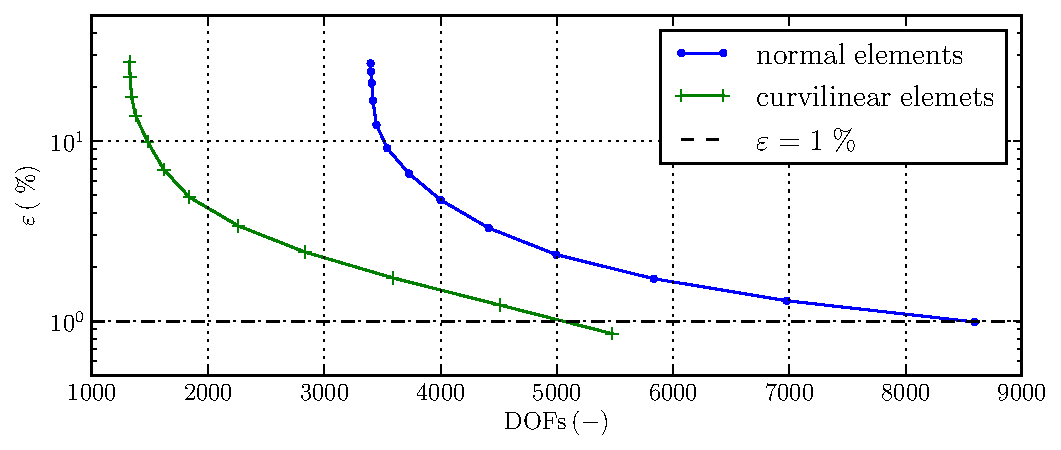
\includegraphics[width=20em]{curvilinear_elements/convergence.pdf}
	\end{minipage}
\end{center}
\vspace{4cm}
}

\headerbox{Adaptivity}{name=adaptivity,column=0,row=0,span=3,below=curvilinear_elements}{
\begin{center}
	\begin{minipage}{20em}
		\centering
		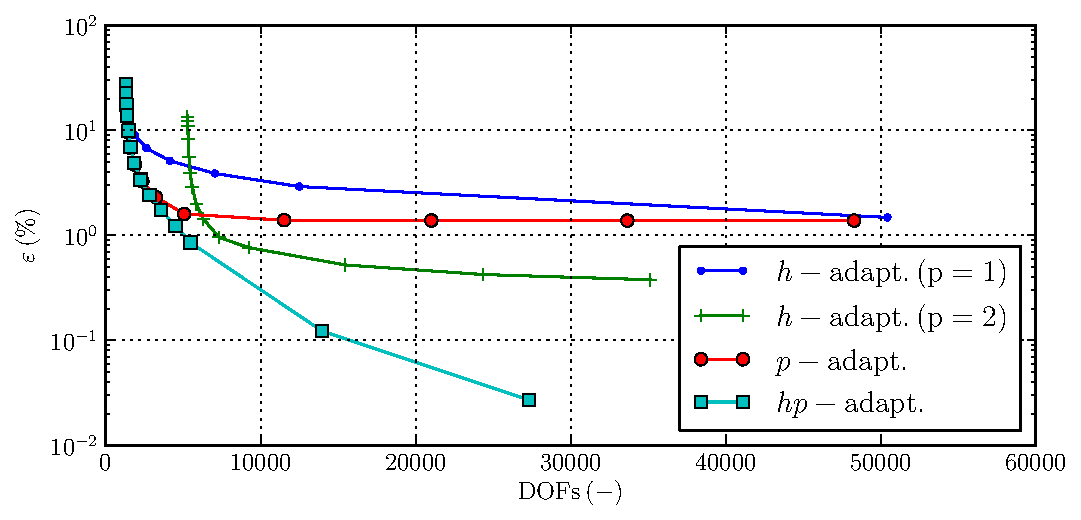
\includegraphics[width=20em]{adaptivity/convergence.pdf}
	\end{minipage}
\end{center}
}

\headerbox{Arbitrary level hanging nodes}{name=arbitrary,column=3,row=0,span=3,below=curvilinear_elements}{
}

\headerbox{Optimization}{name=optimization,column=2,row=0,span=4}{
\begin{center}
        \begin{minipage}{13em}
	    In the engineering practise, the usual demand is not only to calculate some field, 
	    but also to be able to design some of the construction parameters in order to 
optimize some properties. In Agros2D, optimization is possible thanks to scripting -- a python 
interpreter is included.
	\end{minipage}
	\begin{minipage}{4em}
		\centering
		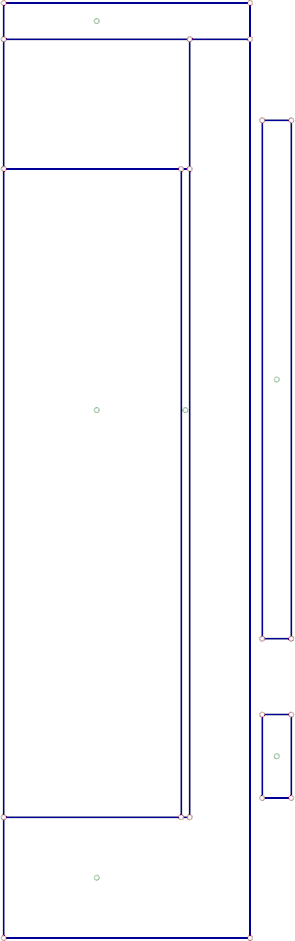
\includegraphics[scale=0.125]{optimization/variant_1.png}
	\end{minipage}
	\begin{minipage}{5em}
		\centering
		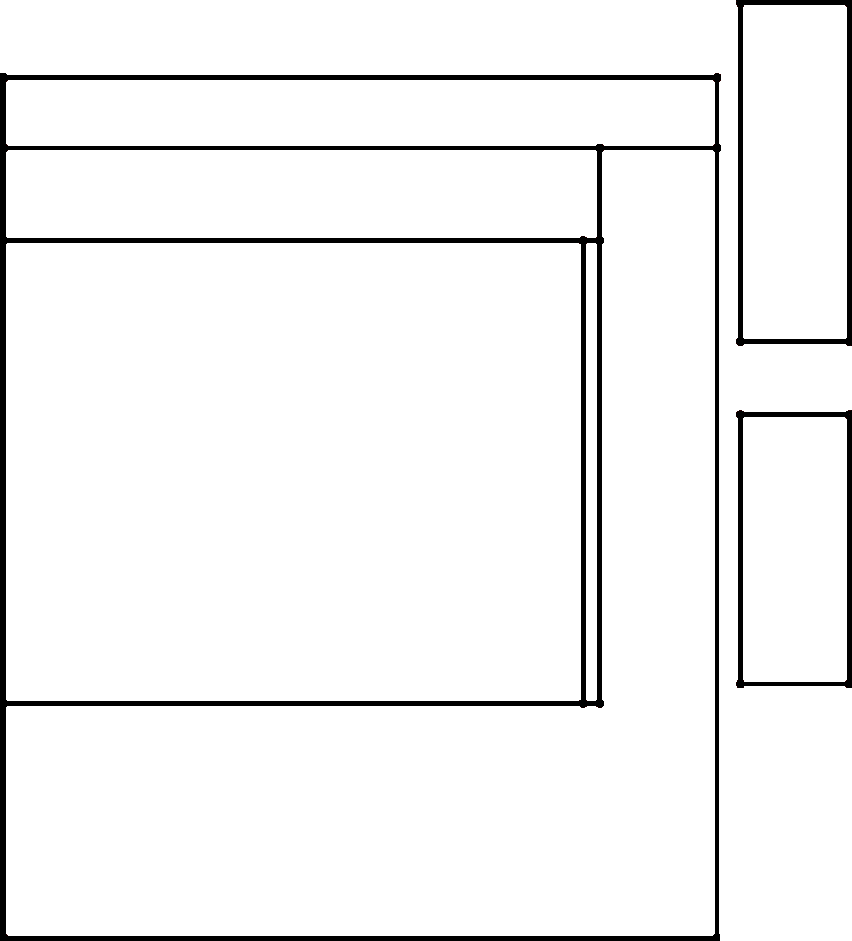
\includegraphics[scale=0.125]{optimization/variant_2.png}
	\end{minipage}
	\begin{minipage}{9em}
		\centering
		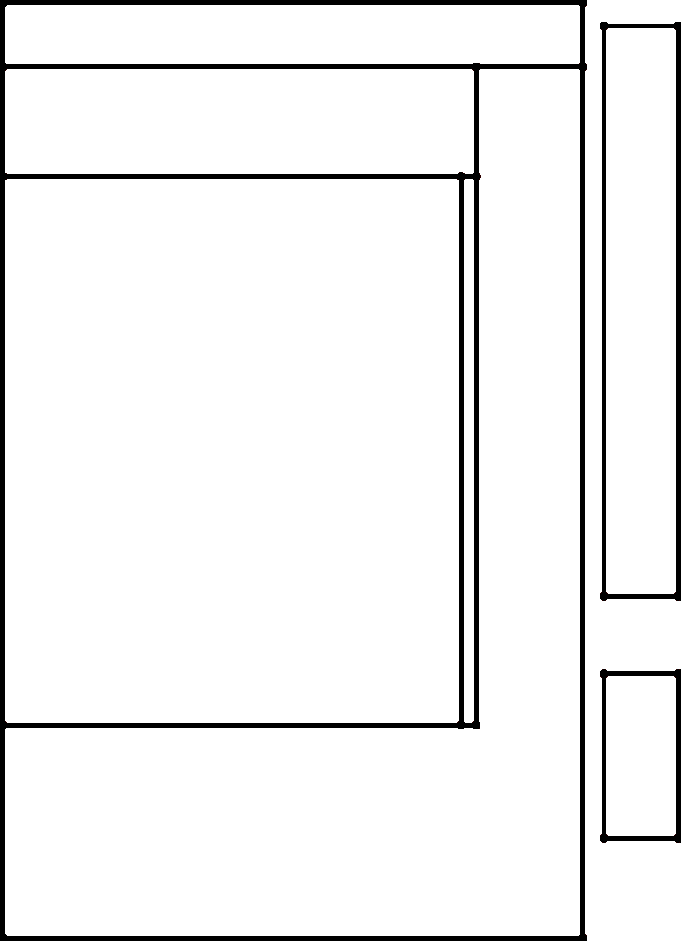
\includegraphics[scale=0.125]{optimization/variant_3.png}
	\end{minipage}
	\begin{minipage}{8em}
		\centering
		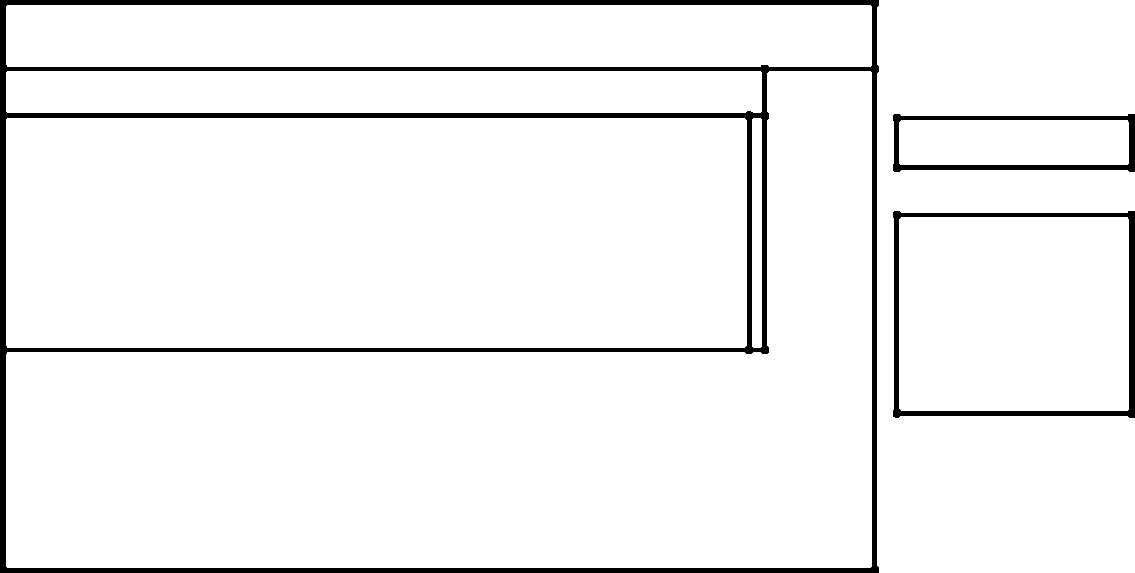
\includegraphics[scale=0.125]{optimization/variant_4.png}
	\end{minipage}
	\begin{minipage}{10em}
		\centering
		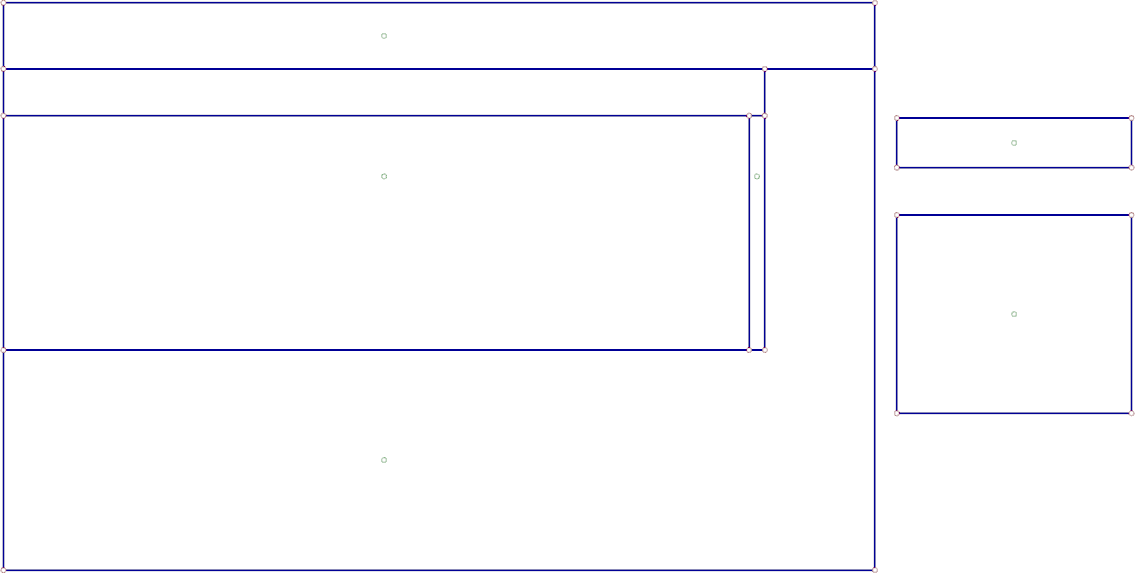
\includegraphics[scale=0.125]{optimization/variant_5.png}
	\end{minipage}
\end{center}

\begin{center}
	\begin{minipage}{12em}
		\centering
		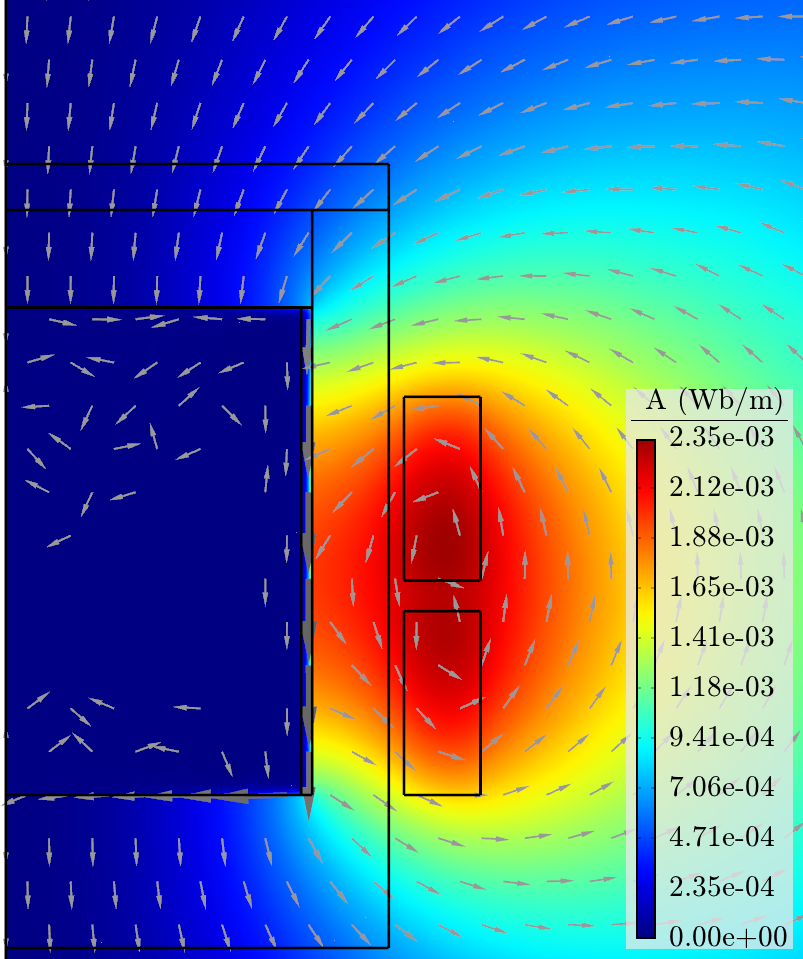
\includegraphics[height=16em]{optimization/magnetic_field.png}
	\end{minipage}
	\begin{minipage}{12em}
		\centering
		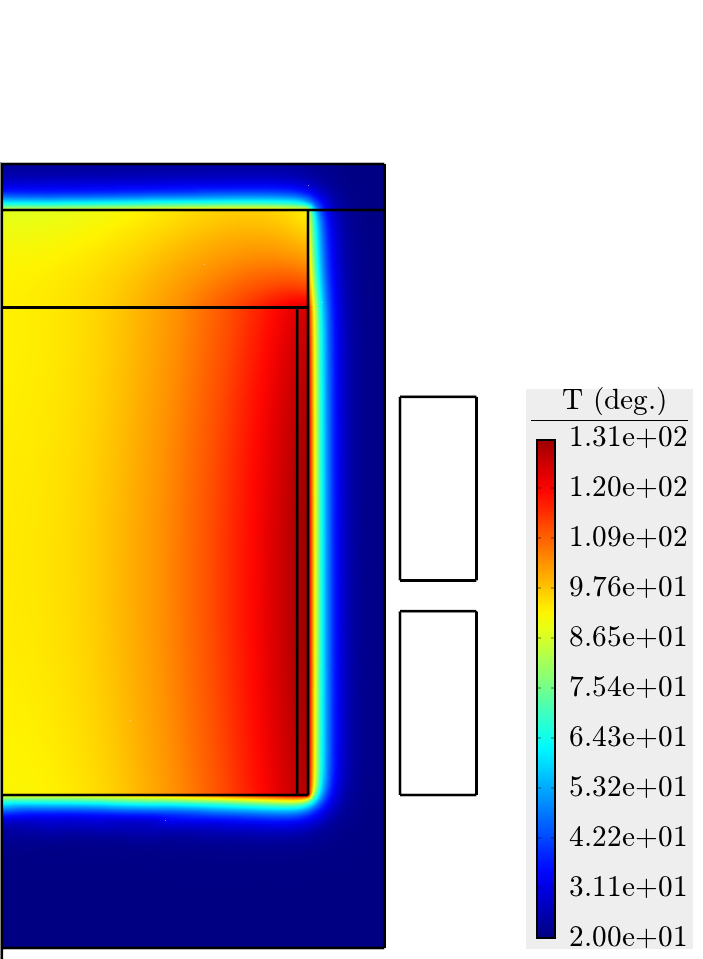
\includegraphics[height=16em]{optimization/temperature_field.png}
	\end{minipage}
	\begin{minipage}{26em}
		In the figure above, we can see several configurations of an owen used for induction heating.
The schema (and also the calculations) are axisymetric.
Several parameters can be changed -- the shape of the owen (height and diameter) can changed, but its volume remains constant.
Also the position and size of inductors (two bars on the right hand side of the figure) can be changed. In the figure left we can 
see magnetic field generated by the inductor and temperature field generated by Joule losses in the material.

	\end{minipage}
\end{center}

\begin{center}
	\begin{minipage}{25em}
		In this problem, there are two different indicators of the quality of the design. First, total heat generated in the 
owen should be as big as possible, and, second, it should be equaly distributed. In the figure, each point represents one calculation 
and its resulting heat $Q$ (should be maximalized) and unevennes of distribution of heat $U$ (shoul be minimalized). Blue points represent
calculations with randomly chosen parameters. Red points are products of optimization (simple implementation of conjugate gradient method has
been used). ...
	\end{minipage}
	\begin{minipage}{25em}
		\centering
		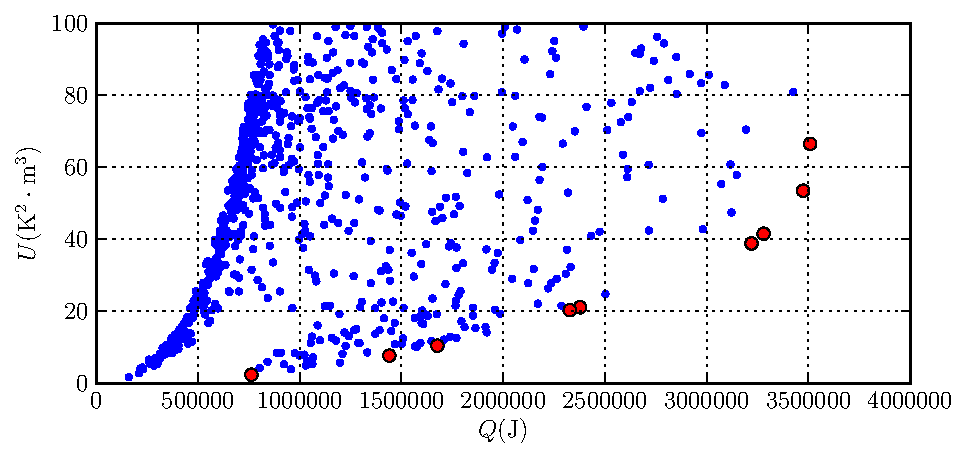
\includegraphics[width=25em]{optimization/results.pdf}
	\end{minipage}
\end{center}
}

\headerbox{Particle tracing}{name=particle_tracing,column=2,row=0,span=4,below=optimization}{
\begin{center}
  \begin{minipage}{17em}
fds dfsfs fdsads ffds fdsfsd fdsfsd fdsfsdf fdsfds fdsfs 
  \end{minipage}
	\begin{minipage}{17em}
	 		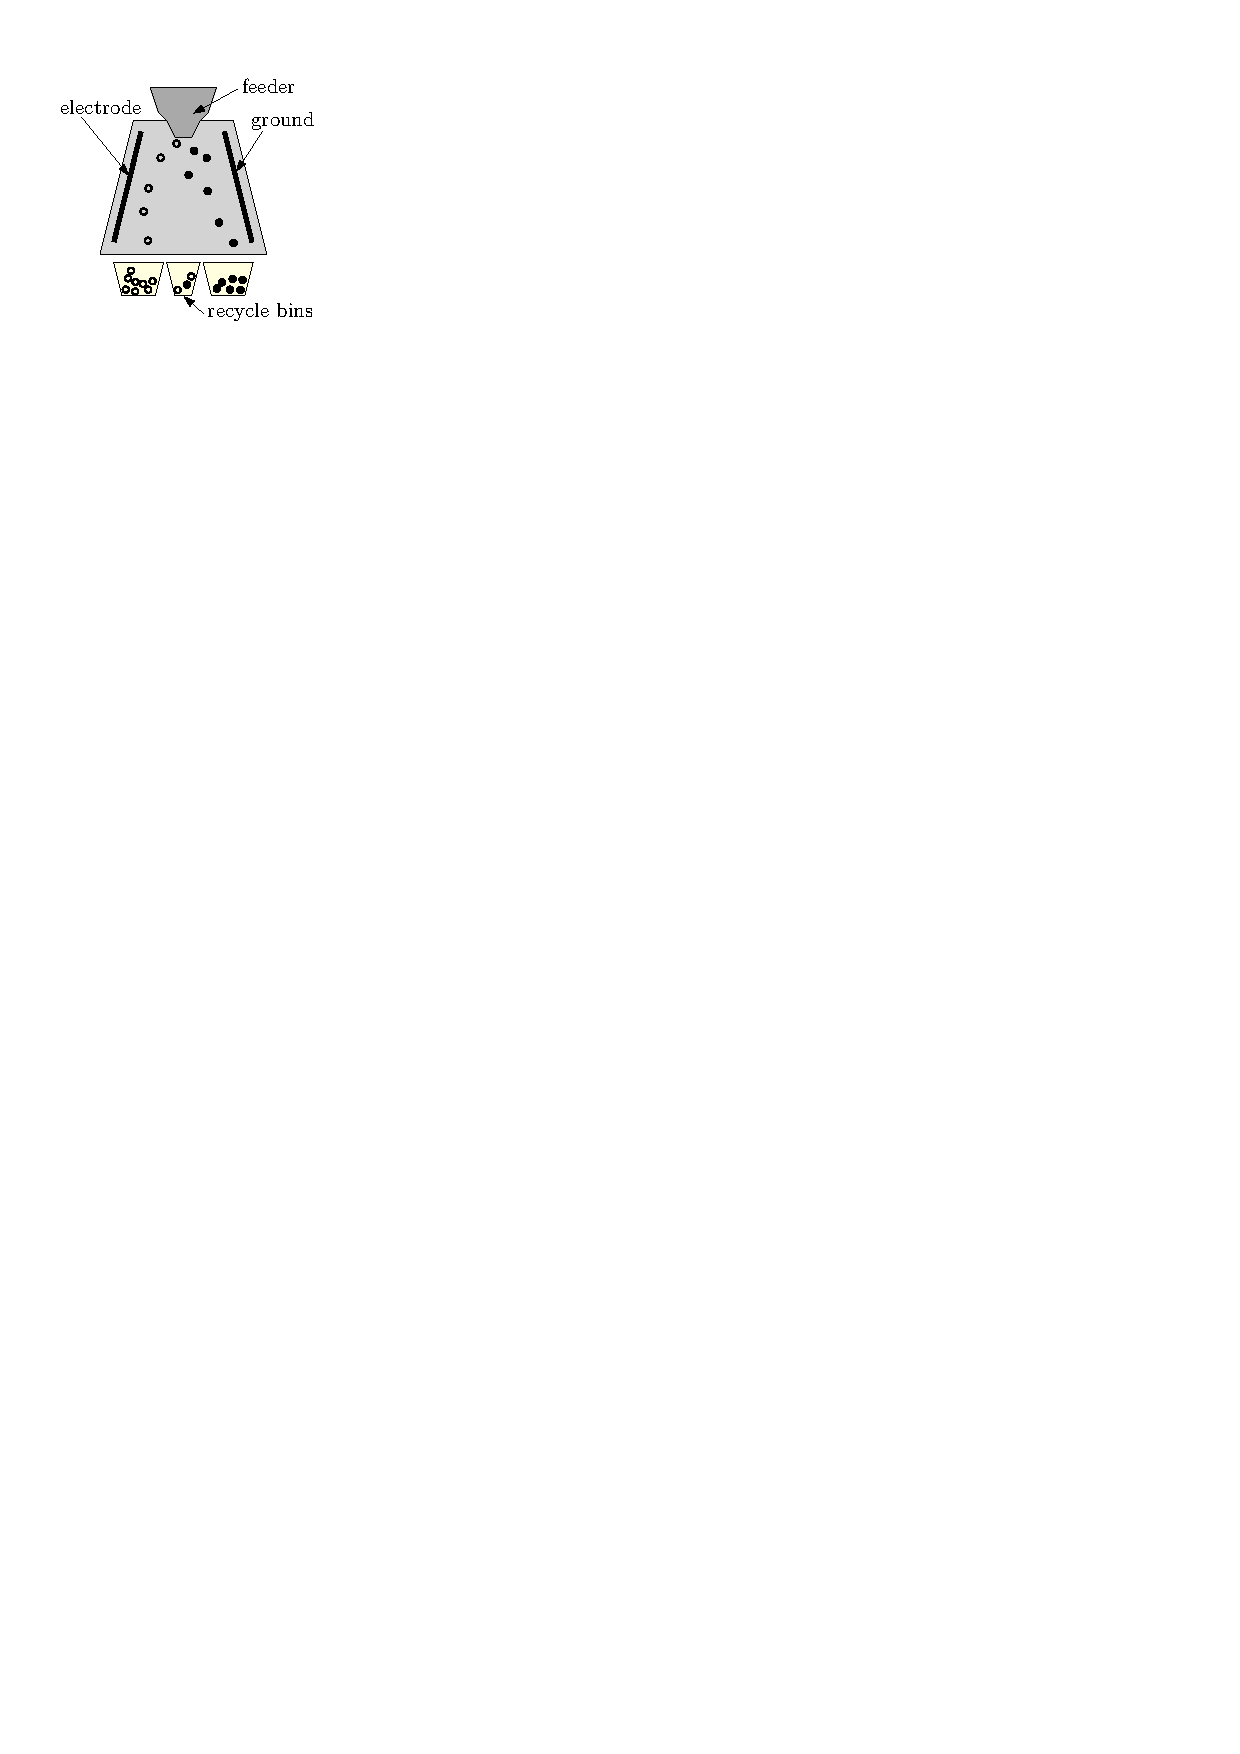
\includegraphics[width=16em]{particle_tracing/princip_pruchod.pdf}
	\end{minipage}
  \begin{minipage}{17em}
fds dfsfs fdsads ffds fdsfsd fdsfsd fdsfsdf fdsfds fdsfs 
  \end{minipage}
\end{center}
%
\begin{center}
	\begin{minipage}{18em}
	 		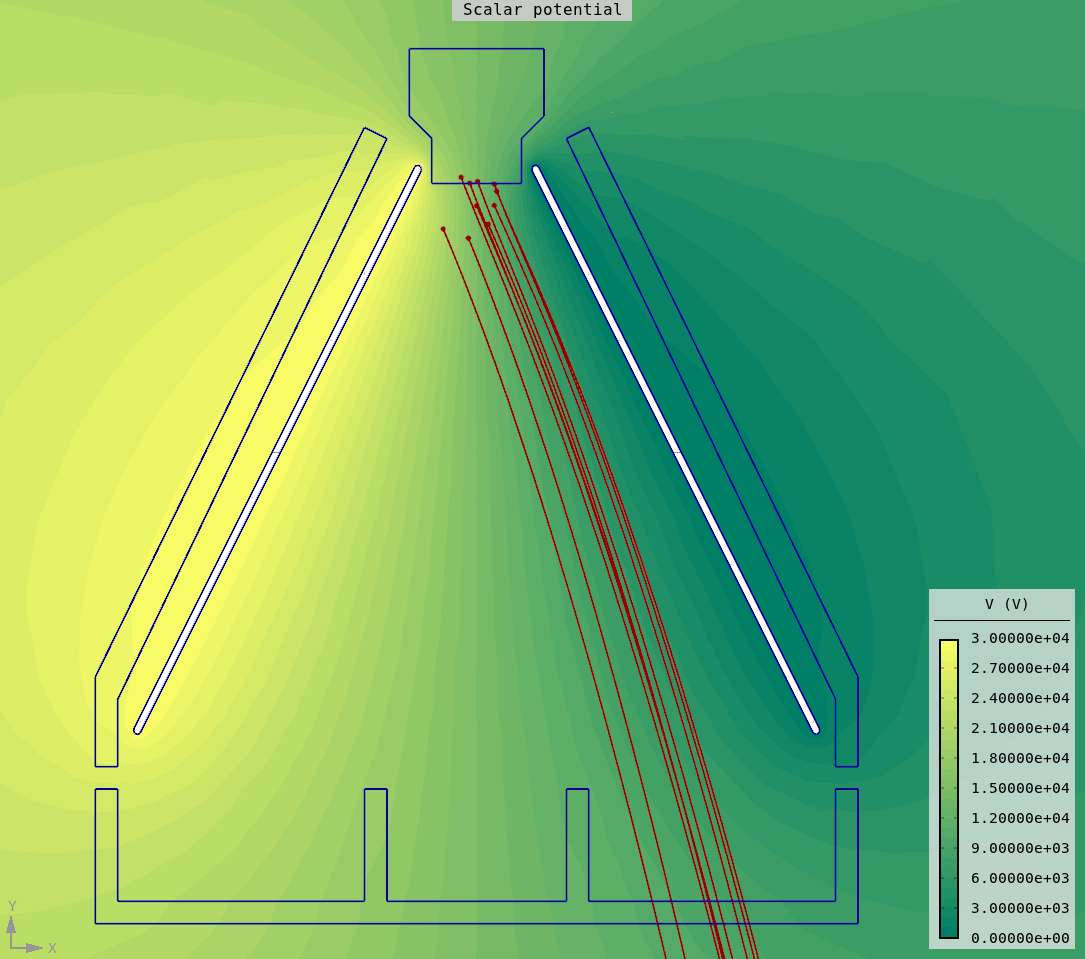
\includegraphics[width=17em]{particle_tracing/separator.png}
	\end{minipage} 
  \begin{minipage}{15em}
fds dfsfs fdsads ffds fdsfsd fdsfsd fdsfsdf fdsfds fdsfs 
  \end{minipage}
	\begin{minipage}{18em}
	 		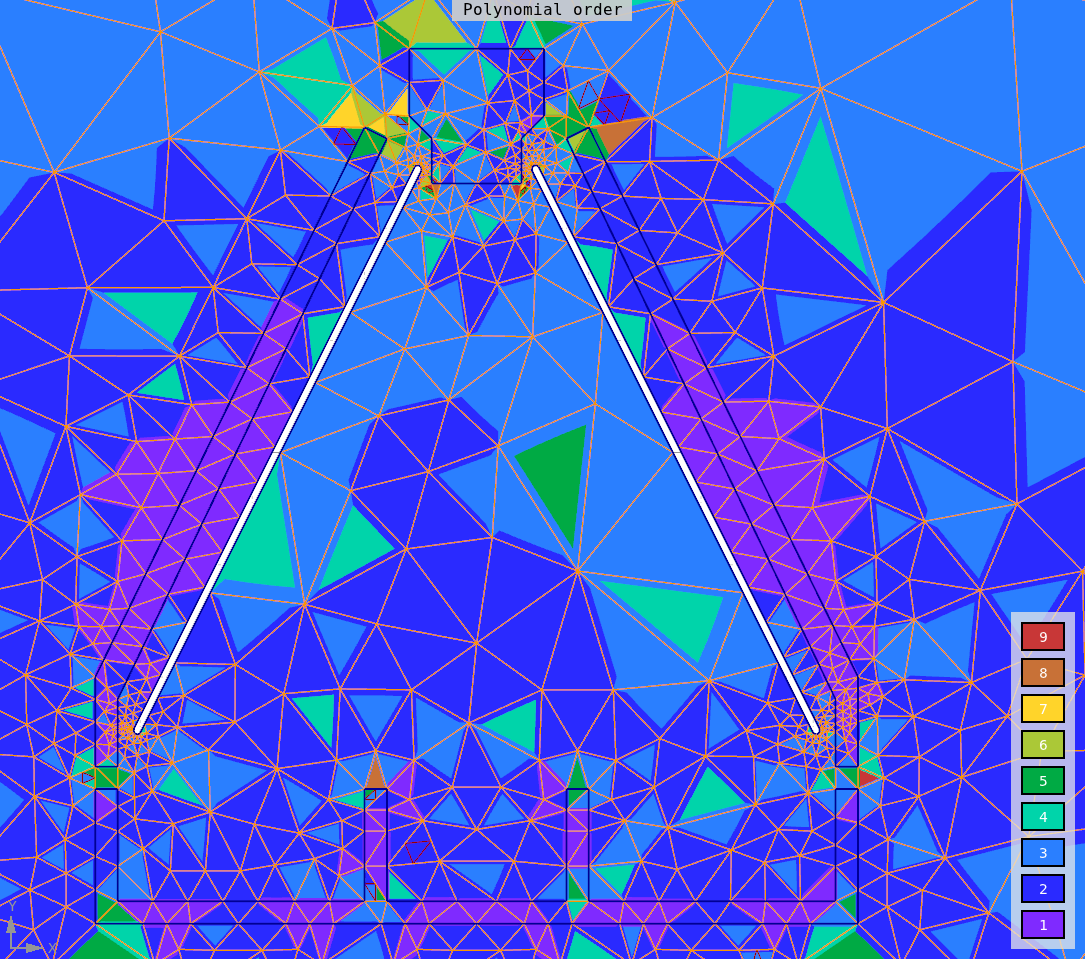
\includegraphics[width=17em]{particle_tracing/separator_sit.png}
	\end{minipage} 
\end{center}


}
\headerbox{References}{name=references,column=0,row=0,span=6,below=particle_tracing, below=adaptivity}{
}
\end{poster}
\end{document}